\documentclass[assignment = 0]{homework}

\usepackage{caption, subcaption, pdfpages, float}
\usepackage{graphics, wrapfig, pgf, graphicx}
\graphicspath{{../imagens/}}


% pacotes para importar código
\usepackage{caption, booktabs}
\usepackage[section, newfloat]{minted}
\definecolor{sepia}{RGB}{252,246,226}
\setminted{
    bgcolor = sepia,
    style   = pastie,
    frame   = leftline,
    autogobble,
    samepage,
    python3,
}
\setmintedinline{
    bgcolor={}
}

% ambientes de códigos de Python
\newmintedfile[pyinclude]{python}{}
\newmintinline[pyline]{python}{}
\newcommand{\pyref}[2]{\href{#1}{\texttt{#2}}}

\SetupFloatingEnvironment{listing}{name=Código}

\usepackage[style=verbose-ibid,backend=biber]{biblatex}
\bibliography{referencias}
\usepackage{csquotes}
\usepackage[noabbrev, nameinlink, brazilian]{cleveref}

\begin{document}

    \section{Introdução}

    O objetivo deste trabalho é de realizar processamentos básicos de imagem e se familiarizar com Python e suas ferramentas. Pensando nisso, o programa desenvolvido utiliza a biblioteca OpenCV para leitura, codificação e decodificação de imagens \texttt{PNG} e usa Numpy para tratamento vetorizado da imagem.

    Todos os processamentos serão aplicados nas mesmas imagens da especificação do trabalho e uma imagem colorida, apresentada na \cref{fig:baboon}.

    \begin{figure}[H]
        \centering
        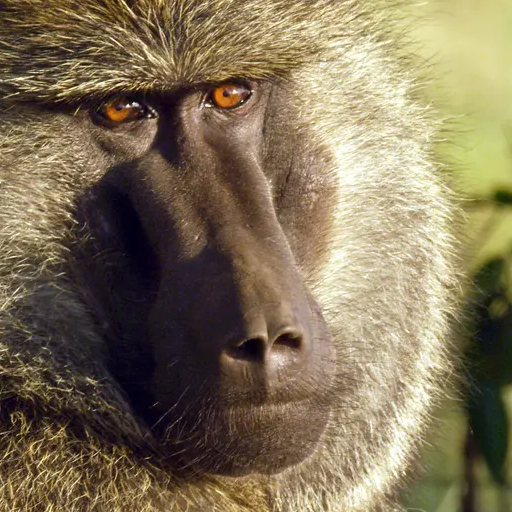
\includegraphics[width=6cm]{color.png}

        \caption{Imagem colorida usada como comparação dos resultados dos processamentos.}
        \label{fig:baboon}
    \end{figure}

    \section{O Programa}

    \subsection{Código Fonte}

    O programa foi desenvolvido em 4 arquivos separados:

    \begin{description}
        \item[main.py] É o corpo do programa, resposável por processar os comandos e opções da linha de comando.

        \item[inout.py] Funções que tratam da entrada e saída do programa, como leitura e escritas de arquivos de imagem e também da apresentação da imagem em uma janela gráfica.

        \item[lib.py] Funções de tranformação da imagem, como ajute de brilho e acesso do plano de bits.

        \item[tipos.py] Definição dos tipos para tipagem estática (apenas o protocolo \autocite{ref:pep544} \pyline{Image}).
    \end{description}

    A tipagem estática é aplicada para facilitar o desenvolvimento e a leitura do código, mas ela limita a execução em Python para as versões 3.7 ou superior \autocite{ref:pep563}.

    \subsection{Execução}

    A execução deve ser feita através do interpretador de Python 3.7+. A única entrada obrigatória é o caminho para a imagem PNG que será processada. As entradas seguintes serão tratadas como comandos de processamento da imagem. Ao final da execução, a imagem resultante será exibida na tela. Por exemplo, o comando abaixo

    \begin{minted}{bash}
        $ python3.8 main.py baboon.png negativo
    \end{minted}

    \subsection{Comandos}
    \subsection{Entrada}
    \subsection{Saída}

    \section{Implementação}
    Cada um? Default pro mosaico?

    \section{Resultados}

\end{document}
